\section{Measurements Procedure}
\subsection{Relaxation time}
In this part of the experiment we study the relaxation times $T_1$ and $T_2$ of samples Gd500 and Gd600. For that we first start by calibrating the magnet of the p20 unit by inserting the Gd600 sample and setting the 90° pulse for it to maximize the received signal. Analogously the 180° is set up for it to minimize the NMR signal. 

After calibration the measurements are taken as previously described: For $T_2$ we use the Hahn echo method and Carr-Purcell metod, whereas for $T_1$ we implement a 180°-90° sequence. 
During the entirety of this measurement the working frequency was set to $\omega_w = (1 \pm 0.5)$ kHz.
\subsection{Chemical shift}
\label{sec: chemical shift}
Next we use the NMR to identify 5 substances. For the identification of the probes we use TMS as a reference substance, hence we have two samples for each probes: one for the unknown substance alone and a second sample mixed with TMS.
The samples are inserted in the magnet of the p20 unit, then the probe are rapidly rotate using compressed air. This procedure was implemented to minimize the field inhomogeneities, hence minimizing the width of the signal in frequency space. Consequently we perform a spin-echo measurement. The signal is Fourier transformed and a Gaussian profile is fitted into the different peaks of the spectrum to measure the frequency of the maxima. These peaks correspond to the active groups of the molecule.
The spectrum of the sample without TMS is compared to the one with TMS to identify the position its corresponding maximum. Finally the relative distance between the TMS-maximum and the active group's maxima is measured. Using Fig. \ref{fig: chemical shift} we are able to identify the active groups. Once these are know we search for the matching molecules in Fig. \ref{fig: identification}.
\begin{figure}[!htbp]
 \begin{center}
  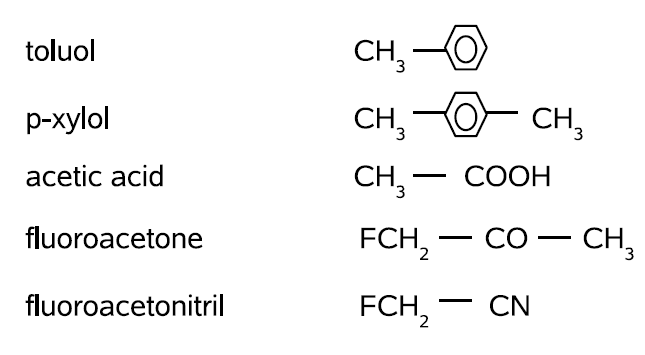
\includegraphics[width = .6\textwidth]{Latex images/molecules.png}
  \caption[]{Five substances for identification \footnotemark}
    \label{fig: identification}
 \end{center}
\end{figure}
\footnotetext{R. Schicker (2021, March 4). Nuclear Magnetic Resonance F61/F62 p. 20}
\subsection{Imaging}
The last part of the experiment consist of 3 small tasks. All of them were performed using a Bruker minispec mq7.5 directly connected to a computer.
\paragraph{1 dimensional imaging}
In this part we introduce three different samples and study their 1 dimensional profiles. 
\paragraph{Time evolution of system}
We prepare a test tube with 15 ml of sand. About 4 ml of oil are poured into the test tube. The prepared vial is quickly placed into the NMRI device. To study the time evolution of this test tube we take different 1 dimensional profiles throughout a time interval. 
\paragraph{2 dimensional imaging}
We place different objects in the NMRI machine and take 2D profile of them. 

